\section{Introduction}
Accurately determining the parameters that describe an experimental turbulent boundary layer (TBL) is crucial to modelling and understanding these flows \citep{titchener2015calculation,pan2020unscented}. In particular, the parameters that can be employed to characterise the mean velocity profile of a TBL can be used, among other purposes, to determine whether a TBL can be considered as well-behaved, (i.e. not in a post-transitional state or affected by non-equilibrium effects) \citep{Chauhan:2009p10824,Sanmiguel:2017JFM}, to compare the results between different experimental or numerical datasets \citep{Schlatter:2009p13969} or to calculate dimensionless numbers that are used to analyse the effect of disturbances such as the inclusion of obstacles or pressure gradients \citep{Clauser:1954p10911,guemes2019flow}. These parameters include quantities such as: the friction velocity $u_\tau$, defined as $u_\tau = \sqrt{\tau_w/\rho}$ (being $\tau_w$ the mean wall-shear stress and $\rho$ the fluid density); the boundary layer thickness $\delta$, which is the wall-normal distance beyond which viscous effects can be considered as negligible; and the freestream velocity $U_\infty$. Among the classical TBL parameters it is also common to define the so-called integral lengths, such as the displacement thickness $\delta^*$ and the momentum thickness $\theta$, providing information regarding the mass and momentum transfer within the boundary layer. The integral lengths are defined for an incompressible flow as,
\begin{equation}
    \delta^* = \int_{0}^{\infty} \left(1-\frac{U}{U_\infty}\right) \,dy;
\end{equation}
\begin{equation}
 \theta = \int_{0}^{\infty} \frac{U}{U_\infty}\left(1-\frac{U}{U_\infty}\right) \,dy.
\end{equation}

being $U = U(y)$ the velocity distribution as a function of the wall-normal coordinate $y$. Since in turbulent boundary layers, $U$ does not {necessarily reach an asymptotic value} at the boundary-layer edge, the previous formulation can be truncated at the boundary layer thickness $\delta$ for its upper integration limit such that,
\begin{equation}
\label{integral}
    \delta^* = \int_{0}^{\delta} \left(1-\frac{U}{U_e}\right) \,dy;~~ \theta = \int_{0}^{\delta} \frac{U}{U_e}\left(1-\frac{U}{U_e}\right) \,dy
\end{equation}
and in consequence the boundary-layer edge velocity is defined as $U_e = U(y=\delta)$.

Using the previously defined TBL parameters, it is possible to generate new figures of merit, such as the shape factor defined as $H_{12}=\delta^*/\theta$ or the skin-friction coefficient $C_f = \tau_w/(\frac{1}{2} \rho U_\infty^2)$, that allow the assessment of the flow regime or discern whether a particular TBL can be considered to be canonical \citep{Chauhan:2009p10824}. Such quantities are used due to their high sensitivity to different boundary and inflow conditions \citep{Chauhan:2009p10824}.

Regardless of the measurement technique, these boundary-layer parameters are  strongly affected by errors due to discretization of the velocity profile, the spacing between the points, the distance of the first point from the wall, and uncertainty in the wall location \citep{titchener2015calculation,Orlu:2010p36071}. In addition to these sources of error, there is no consensus when it comes to the methodology for calculating $\delta$. Several of the proposed methods rely on the use of additional quantities besides the mean velocity profile, such as the mean vorticity \citep{spalart1993experimental}, the mean streamwise variance \citep{Vinuesa:2016is} or a reference pressure \citep{griffin2020general}. On the other hand, accurate determination of friction-related quantities (such as $u_\tau$ and $\tau_w$) is also particularly challenging \citep{orlu2020instantaneous}. Different experimental approaches that can be employed to measure these quantities, such as oil-film interferometry \citep{Vinuesa:2016tn}, Preston tube \citep{head1962preston},  MEMS shear-stress sensor \citep{sheplak2004mems}.

For {the particular case of zero-pressure gradient (ZPG) TBLs and in} those situations where only mean streamwise velocity measurements are available, an alternative to calculate all the boundary-layer parameters is to resort to composite velocity profiles based on analytical expressions \citep{Chauhan:2009p10824,Coles:2006p898,Nickels:2004p15662,Rodriguez-Lopez2015}. This methodology is based on assuming that the mean streamwise velocity profile can be described using a function that takes the form of $U^+(y^+)= U^+_{inner}+U^+_{outer}$, which is used to fit the data of the aforementioned profile. In the present study the superscript $+$ denotes inner scaling, which is defined as $U^+=U/u_\tau$ and $y/\ell^*$, being $\ell^*$ the viscous length $\ell^* = \nu/u_\tau$ and $\nu$ the kinematic viscosity. The term $U^+_{inner}$ is the part of the function that provides a description of the velocity profile from the viscous sublayer up to the overlap region, while the term $U^+_{outer}$ is used to define the outer region of the TBL profile. The $U^+_{inner}$ function is typically based on $U^+=y^+$ for the inner region and on the logarithmic law $U^+=\frac{1}{\kappa}y^+ +B$ for the overlap region, where $\kappa$ is the von Kármán constant and $B$ is an integration constant. The $U^+_{outer}$ function was introduced by \citet{Coles:2006p898} with the inclusion of the wake function $\mathcal{W}$, defining the wake component of the velocity profile. There are different formulations of the wake function since the wake component is greatly affected by boundary or initial conditions. Depending on the study, the complexity of the $U^+$ formulation can be varied and even some of the parameters can be previously defined from established correlations to reduce the dimensionality of the fitting process. The major advantage of this methodology is that, by using just a full-resolution mean velocity profile, it is possible to estimate the {boundary-layer} parameters and to correct the wall location. 

Hardware and software advances have recently opened the path to full-resolution {TBL velocity-profile} measurements at sufficiently large friction Reynolds number using Particle Image Velocimetry (PIV). In particular, techniques based on ensemble averaging (e.g. single-pixel correlation \citep{westerweel2004single}, or ensemble particle tracking velocimetry, EPTV \citep{cowen1997hybrid,kahler2012uncertainty}) are able to achieve a sufficiently large dynamic range to resolve the entire velocity profile, from the viscous sublayer up to the freestream, thus enabling {composite-profile} application. Single-pixel correlation is based on ensemble averaging of cross-correlation maps. EPTV is based on identifying vectors from instantaneous realisation and superposing them to build a dense cloud of vectors. Statistical information is then inferred from the pdf of the velocity vectors in averaging windows, referred as \textit{bins} (either isotropic, anisotropic or with shape adapted locally \citep{raiola2020adaptive}). 
Reynolds stresses can also be measured accurately if velocity gradient effects within the averaging bin are taken into account. In single-pixel correlation, this can be achieved by proper modelling of the shape of the cross-correlation peak \citep{scharnowski2012reynolds}, while in EPTV the velocity-gradient effect can be reduced by local polynomial fitting of the vectors to be averaged \citep{aguera2016ensemble}. It was recently shown in mild {adverse-pressure-gradient TBLs} \citep{SanmiguelVila2017} that this second approach is generally more robust; furthermore, the recent advances in volumetric velocimetry \citep{discetti2018volumetric} are now pushing towards a widespread use of Lagrangian Particle Tracking (LPT), thus motivating an increased interest in understanding the capabilities of EPTV approaches in measuring velocity profiles. PIV/PTV offer the indisputable advantage of providing also information on the instantaneous flow field organisation; this renders worth exploring the uncertainty of PIV/PTV/LPT in determining parameters which are normally measured using the portfolio of techniques mentioned above.

In this work, the uncertainty in extracting boundary-layer parameters from ``full-field'' EPTV data is explored, i.e. assuming that the field of view covers the entire {boundary-layer} thickness plus a robust freestream measurement. {For the sake of simplicity, the present study is focused on well-behaved ZPG TBLs in which a composite-profile approach can be applied, as in hot-wire measurements.} While it is common to use separate experiments for high-resolution near-wall measurements (see for instance the work by \citet{kahler2006wall}) and for the {full-field} organisation, the approach we present here has the advantage of requiring the same image dataset for statistics extraction and flow field characterisation.
We will first simulate in virtual experiments the effect of finite spatial resolution on data generated from Direct Numerical Simulations (DNS) of a {ZPG TBL} and using a composite profile {formulation of a ZPG TBL}. Systematic errors due to the bin-averaging effect and the position of the first measurement point with respect to the wall are addressed in \S \ref{s:SyntheticValidation} as a function of the bin size. {In this section random errors due to finite convergence or wall-positioning uncertainty are not introduced, as the focus is simply on systematic error.}

Then {in \S \ref{s:validation}} a {Monte Carlo} study is conducted to estimate the uncertainty of the composite profile fitting due to finite number of samples. This is particularly relevant in EPTV, since the bin size depends on the number of snapshots and the number of vectors within the bin, considered sufficient for a satisfactory accuracy. {The method will thus deliver an uncertainty range for each turbulent-boundary-layer parameter. An experimental validation is carried out to verify that the error on the ZPG TBL parameters are predicted within an uncertainty range for a wide range of bin sizes.} 

%--------------------------------------------------------------------------------
%------------------------------- METHODOLOGY ------------------------------------
%--------------------------------------------------------------------------------
\section{Methodology}
The methodology to estimate the uncertainty of EPTV measurements for TBL characterisation is illustrated in this section. The method is based on simulating the errors due to finite resolution and convergence on existing TBL profiles, either based on DNS {ZPG} data or on analytical formulation of {ZPG TBL} composite profiles. Different levels of camera resolutions and bin sizes are explored in order to investigate systematic errors in the fitting procedure and the random uncertainty due to convergence issues. {In the proposed method no particle images are generated; the effects of the error sources are directly simulated by averaging existing velocity profiles (or generated ad hoc with composite profile formulations). This renders the method of simple and general application, avoiding the need of generating virtual images for the specific case.}

\subsection{Synthetic profile generation} \label{ss:synthetic_method}

The synthetic TBL profile is generated from existing datasets to replicate the incurred errors from experiments using EPTV. The synthetic profile is generated using as a reference:

\begin{itemize}
    \item Dataset of {ZPG TBL} DNS simulations, available in the turbulent database of the Fluid Dynamics Group from Universidad Politécnica de Madrid\footnote{\url{https://torroja.dmt.upm.es/turbdata/blayers/}}. In particular, for the analysis conducted in the following, the data corresponding to $Re_{\vartheta}=4500$ have been used \citep{sillero2013one}.
    \item Composite-profile generated data based on the ZPG TBL formulation by \citet{Chauhan:2009p10824} which will be briefly outlined in \S \ref{s:composite_profile}.
\end{itemize}

{The velocity vectors are directly generated from the interpolation of the DNS data in the first case, and from the analytical formulation of the composite profile in the second case.} In all cases, the simulated field of view spans from the wall to $1.3\delta$. This upper bound is set in order to guarantee a sufficiently robust measurement of the freestream. The resolution is here defined in wall units as {$Res = \frac{S}{1.3 Re_\tau}$}, being $S$ the available pixels in the camera sensor in the wall-normal direction. 

The systematic error due to bin averaging in the binning process of the EPTV is simulated by top-hat averaging of the velocity profiles within bins of different size. We tested bin sizes ranging between {$1\ell^*$ to $200\ell^*$}. The bin size distribution in wall units is reported in Figure \ref{fig:window} as a function of the size in pixels and of the spatial resolution expressed in pixels per wall unit.

The profiles are truncated removing from the near-wall region bins which were not completely included in the domain. While this would imply removing vectors with distance from the wall smaller than one half of the window size, after the analysis of the experimental results, we decided to introduce a more restrictive criterion and cut the profiles to a distance of 3/4 of the window size. This criterion excludes from the analysis pixels in close proximity from the wall, which are very likely to be affected by spurious reflection effects in PIV measurements. Due to the sensitivity of the composite-profile formulation to the quality of the near-wall data, this criterion was found to be more robust. 

The effect on the streamwise mean velocity profile of the bin averaging is shown in Figure~\ref{fig:F1_DNSprofiles} for DNS data. The effect of increasing the bin size is clear in the near-wall region, where the measured profile departs from the baseline due to averaging effects. It is expected that this systematic error, combined with the lack of points in the near-wall region for relatively large bin size, will yield more significant errors in determining the friction velocity and the wall position. Also, the computation of integral quantities is sensitive to the position of the nearest point to the wall \citep{titchener2015calculation,Rodriguez-Lopez2015}. 

\begin{figure}
    \centering
    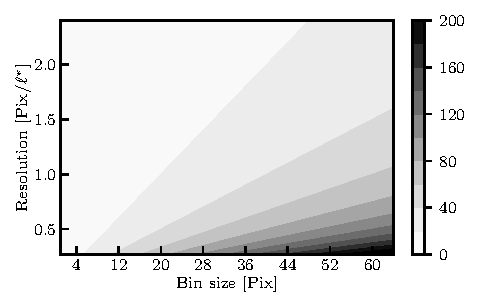
\includegraphics[width=0.75\columnwidth]{Figures/figure08.pdf}
    \caption{Bin size distribution {expressed in wall units $l^*$} with respect to bin size in pixels and resolution.}
    \label{fig:window}
\end{figure}


\begin{figure}
    \centering
    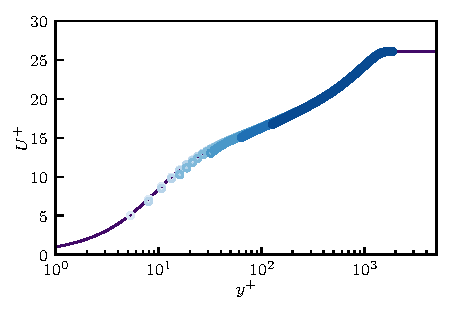
\includegraphics[width=0.75\columnwidth]{Figures/figure05.pdf}
    \caption{Effect on the streamwise mean velocity profile of the bin averaging in EPTV with 2 \sy{blue1}{o}, 4 \sy{blue2}{o}, 8 \sy{blue3}{o}, 16 \sy{blue4}{o}, {32} \sy{blue5}{o}, and 64 \sy{blue6}{o} pixels bin size for a fixed value of $S=700$. Ground truth DNS data is referred as \lcap{-}{dark}.}
    \label{fig:F1_DNSprofiles}
\end{figure}

Two contributions of random error have been included. The first error is a perturbation of the initial guess of the wall position, which is most often inferred from visual inspection of the images. This process might be severely affected by the image quality near the wall; furthermore, depending on the surface material and quality, the wall position might not be completely clear. {Throughout this work} we introduced a uniformly distributed random error with bounds $\pm0.5$ pixels, even though the presented uncertainty estimation method can be tuned to model more optimistic/pessimistic scenarios. The second contribution of random error is due to convergence, which depends on the random error on the velocity vectors (assumed here having Gaussian distribution with standard deviation $\sigma_v$) and on the turbulent fluctuation levels. If we indicated with $u'$ the standard deviation of the streamwise turbulent fluctuations, the expected standard deviation of the error of the mean is:
\begin{equation}
\label{ruido}
    \sigma_{U}=\frac{\sqrt{u'^2+\sigma_v^2}}{\sqrt{N_v}}    
\end{equation}
with $N_v$ being the number of vectors in each bin (supposing for simplicity it is sufficiently small to ensure that on average it contains less than 1 vector per snapshot). 
For the DNS data, the profile of $u'$ is available and can be directly plugged in Eq.~\ref{ruido}; however, for the case simulated with the composite profile proposed by \citet{Chauhan:2009p10824}, since an analytical formulation for second-order statistics is not readily available, the standard deviation of the error of the mean is modelled assuming a two-level distribution with piecewise constant $u'$. A level of $u'^+=2$ for $y<0.9 \delta$ is chosen as an average value of the streamwise turbulent fluctuations for the $Re_\tau$ under study and a value of $u'^+=0.5$ as a representative value of the freestream velocity is used for the locations $y\geq 0.9 \delta$.

A {Monte Carlo} approach is followed to characterise the uncertainty on the estimation of the {ZPG }TBL parameters. The systematic and random uncertainty are defined respectively using the median and the standard deviation of the results of the simulated experiments. {The systematic errors are addressed in \S \ref{s:SyntheticValidation}, while the effect on random uncertainty is introduced in \S \ref{s:validation}.}

\subsection{Calculation of the boundary-layer parameters}
\label{s:composite_profile}

In order to calculate the different boundary-layer parameters and to correct the wall location using only the mean streamwise velocity profile, a two-step strategy based on the use of two different composite profiles is followed. In a first step, the mean velocity data after the EPTV process is fitted to the composite profile proposed by \citet{Chauhan:2009p10824} {for ZPG TBLs }and defined as follows,

\begin{equation} \label{eq:chauhan}
U^+=U^+_{inner}+\frac{2\Pi}{\kappa} \mathcal{W} \left( \eta \right), 
\end{equation}
being $\Pi$ the wake parameter and $\eta=y^+/\delta^+$. Using this formulations the $U^+_{inner}$ and $\mathcal{W}\left(\eta \right)$ read as follows,

\begin{equation}
\label{innerchuahan}
\begin{array}{ll}
U^+_{inner}=& \frac{1}{\kappa} \ln\left(\frac{y^+-a}{-a}\right)  + \frac{R^2}{a(4\alpha+a)} 
 (4\alpha+a)  \\
& \left[ \ln \left(-\frac{a}{R}\frac{\sqrt{(y^+ -\alpha)^2+\beta^2}}{y^+-a}\right) +\frac{\alpha}{\beta}(4\alpha+5a) \right. \\
& \left. \left(\arctan\left(\frac{y^+-\alpha}{\beta}\right)+\arctan\left(\frac{\alpha}{\beta}\right)\right) \right]+ \\ &\frac{\exp[-\ln^2(y^+/30)]}{2.85},
\end{array}
\end{equation} 
where $\alpha=(-1/\kappa-a)/2$, $\beta=\sqrt{-2a\alpha-\alpha^2}$, $R=\sqrt{\alpha^2+\beta^2}$, $\kappa=0.384$ and $a=-10.3061$. The wake function $\mathcal{W}$ is defined as,

\begin{equation}
\label{outerchauhan}
\begin{array}{ll}
\mathcal{W}(\eta)= & \frac{1-\exp\left[-(1/4)(5a_2+6a_3+7a_4)\eta^4+a_2\eta^5 +a_3\eta^6+a_4\eta^7
	\right]}{1-\exp[-(a_2+2a_3+3a_4)/4]}  \\
& \times \left(1-\frac{1}{2\Pi}\ln(\eta)\right) 
\end{array}
\end{equation} 
where $a_2=132.8410$, $a_3=-166.2041$ and $a_4=71.9114$. The values of the constants have been derived by \citet{Chauhan:2009p10824} from several experiments over a large Reynolds number range and their formulation has been tested and proved to be robust when it comes to identify well-behaved profiles  \citep{Chauhan:2009p10824}. This composite-profile formulation is used to determine the values of $u_\tau$ and to correct the absolute wall position correction $\Delta y $ by means of a least-square procedure \citep{Chauhan:2009p10824,Orlu:2010p36071,Rodriguez-Lopez2015}. Since the values of the constants are fixed, this formulation allows to calculate $u_\tau$ without relying on locating the overlap region.

In the second step, the extracted values of $u_\tau$ and $\Delta y$ are used to calculate the corresponding $U^+$ and $y^+$ and then fit them to the composite profile proposed by \citet{Nickels:2004p15662}, which has the following formulation for the particular case of a {ZPG TBL}, 

\begin{equation}
\label{Nickels}
\begin{array}{lll}
U^+ = & y^+_c \left[1- (1+2(y^+/y_c^+)+\frac{3}{2}(y^+/y^+_c)^2)e^{-3y^+/y_c^+}  \right] \\
& \times \frac{1}{6\kappa
_0} \left(\ln(\frac{1+(0.6(y^+/y_c^+))^6}{1+\eta^6})+b(1-e^{-\frac{5(\eta^4+\eta^8)}{1+5\eta^3}})\right) 
\end{array}
\end{equation} 
in which $b$ is a measure of the wake strength and is equivalent to wake parameter, $\kappa_0=0.39$ and $y_c^+=12$. 
This composite profile is used for the calculation of the edge velocity $U_e$ and the boundary-layer thickness $\delta$ because of its description of the wake region. The wake function proposed by \citet{Nickels:2004p15662} has been proved to be robust at low Reynolds numbers for both experimental and numerical profiles \citep{Schlatter:2010p35519}. Eventually, the resulting fitted velocity profile is integrated according to Eq.~\ref{integral} and using the $\delta$ and $U_e$ for the integration limits to extract $\delta^*$ and $\theta$. 

\section{Systematic error estimation for synthetic data}
\label{s:SyntheticValidation}

\begin{figure}
    \centering
    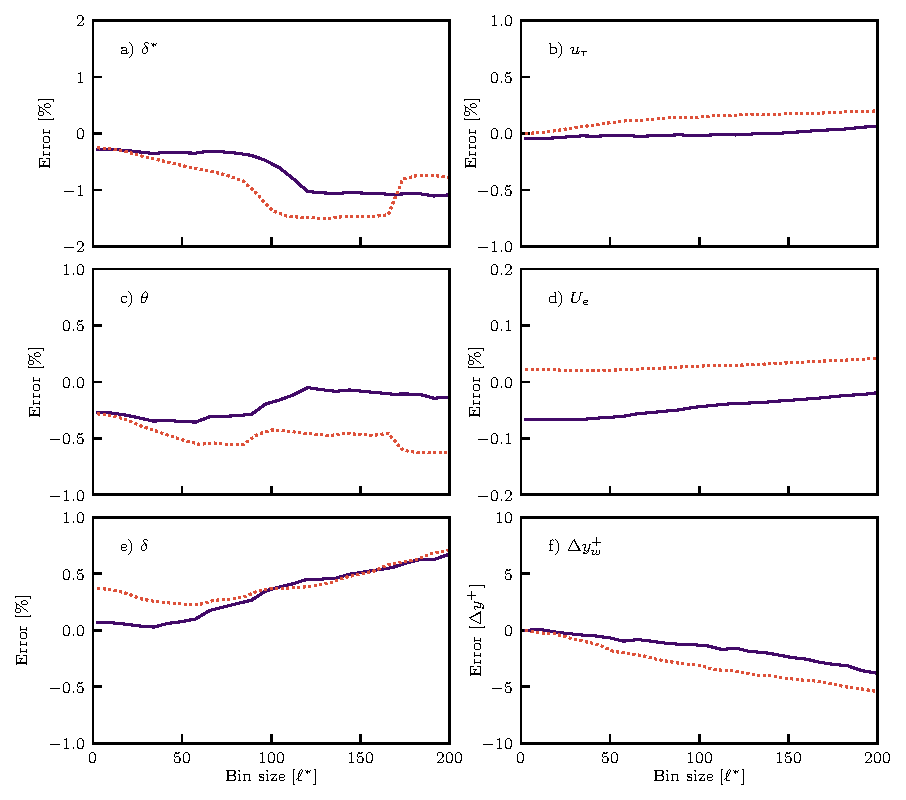
\includegraphics[width=\textwidth]{Figures/figure09.pdf}
    \caption{Systematic error as a function of the bin size for a) displacement thickness, b) friction velocity, c) momentum thickness, d) freestream velocity, e) boundary layer thickness, and f) y origin. Symbols refer to DNS \lcap{-}{dark}, Composite-profile \lcap{:}{purple}.}
    \label{fig:systematic_error}
\end{figure}

The procedure described in \S\ref{ss:synthetic_method} is explored {for different bin size in wall units}. {The objective of this section is to explore the systematic error due to the filtering effect on the profile due to finite bin size.} For this reason, the error sources due to convergence and to the wall-normal coordinate are not considered. Therefore, {the computation of TBL parameters} is performed {averaging on} a reduced set of {50} cases with a small random perturbation on the velocity profile ($N_v \sim O(10^6)$) to avoid bias errors due to locking in local minima in the fitting optimization procedure described in \S\ref{s:composite_profile}.

As reported in Figure~\ref{fig:F1_DNSprofiles}, the size increase of the averaging bin promotes two main effects on the velocity profile: the suppression of valid points in the near-wall region based on the criterion describes in \S\ref{ss:synthetic_method}; and the diversion of the near-wall points of the profile. 
As the {bin} size increases, at certain point, the averaging process in the logarithmic region will be affected by points within the buffer region, which eventually tend to curve the profile. As a consequence, the slope of the velocity profile in the logarithmic region will not follow the logarithmic law. This strongly affects the fitting procedure proposed by \citet{Chauhan:2009p10824}, especially for a proper estimation of the wall location and the friction velocity, since it assumes a velocity profile which fulfils the logarithmic law of the wall.

An overview of the performed parametric study is reported in Figure~\ref{fig:systematic_error}, based on data generated according to DNS of a TBL and the composite profile described in \S\ref{s:composite_profile}, respectively. The relative error is computed with respect to the reference parameters reported in Table~\ref{tab:1}.

The systematic error {profiles as a function of the bin size in wall units} are overall consistent between DNS and composite-profile data. This is particularly interesting since the composite profile can be easily generated for conditions matching the experiments, while high-fidelity simulations data might not be available, especially at high Reynolds numbers.

For the parameters computed from the first fit based on \citet{Chauhan:2009p10824}, i.e. $u_\tau$ and $\Delta y^+$, we observe a clear tendency of increasing magnitude of the error as the averaging bin increases in size. Nonetheless, the systematic error in $u_\tau$ estimation does not exceed 1\% and the correction of wall-normal coordinate is below $5^+$ for bin size smaller than {100}$\ell^*$. This result {suggests} that, although the bin size will affect the performance in the estimation of the parameters, the composite profile proposed by \citet{Chauhan:2009p10824} is robust in the inner region of the velocity profile. Only when the bin size affects the logarithmic layer, the fit is not capable of correcting for the wall position with an acceptable level of accuracy. {It is important to remark here that the estimation of $u_\tau$ with the composite profile is robust since the data correspond to ZPG conditions. In presence of pressure-gradient, curvature, roughness or other effects it is well known that the composite profile is less robust and the availability of points in the near-wall region becomes of paramount importance.} 

For the TBL parameters estimated in the second step by using the fit proposed by \citet{Nickels:2004p15662}, we find $\delta^*$ and $\theta$, with a relatively low error for {bin} sizes that lie below the logarithmic region; however, as the bin size exceeds 50$\ell^*$, the error becomes more significant. This is a direct consequence of the curvature smoothing effect promoted by the top-hat averaging as shown in Figure~\ref{fig:F1_DNSprofiles}, which is reducing the effectiveness of the second {inner} fit. Additionally, we find a systematic overestimation of both $\delta$ and $U_e$ {for the composite-profile case (although for the case based on the DNS profile $U_e$ appears to be slightly underestimated)}. This might be surprising at a first glance, since averaging effects are much less relevant at the edge of the boundary layer. This suggests that the truncation and bias errors in the near-wall region of the TBL are also affecting the results of the composite-profile fitting in the outer region. 

\begin{table}
\centering
% table caption is above the table
\caption{\centering Reference TBL parameters for DNS, composite profile and experiments.}
\label{tab:1}       % Give a unique label
% For LaTeX tables use
\resizebox{\textwidth}{!}{%
\begin{tabular}{lcccccccccc}
\hline\noalign{\smallskip}
 Case & $Re_{\tau}$ & $Re_{\theta}$ & $H_{12}$ & $\delta^*/\delta$ & $\theta/\delta$ & $u_{\tau}$[m/s] & $U_{e}$ [m/s] & $\delta$ [mm]  & $\ell^*$ [$\mu$m] & $C_f \cdot 10^3$\\
\noalign{\smallskip}\hline\noalign{\smallskip}
DNS          & 1437 & 4500 & 1.381 & 0.169 & 0.122 & - & -& - & - & 2.98 \\
{Composite-profile}        & 1445 & 4503 & 1.375 & 0.165 & 0.120 & 0.70  & 18.14 & 32 & 22 & 2.98\\ 
Experiments          & 1379 & 4432 & 1.390 & 0.170 & 0.123 & 0.042 & 1.11 & 29 & 21 & 2.91\\
\noalign{\smallskip}\hline
\end{tabular}}
\end{table}

\section{{Random uncertainty measurements - }experimental Validation} \label{s:validation}

{In this section the capabilities of the proposed methods to estimate the uncertainty range of each TBL parameter are tested. For this purpose, differently to the previous section, random errors on the velocity profiles due to finite convergence and wall-positioning are included, with a number of vectors per bin matching experimental conditions. A large number of tests is carried out to obtain statistics of the errors on the TBL parameters, thus delivering uncertainty ranges for each of them. An experimental validation is carried out using a high-resolution ZPG-TBL measurement as ground truth, and investigating the error introduced when increasing the bin size.}

\subsection{Experimental setup}

\begin{figure}
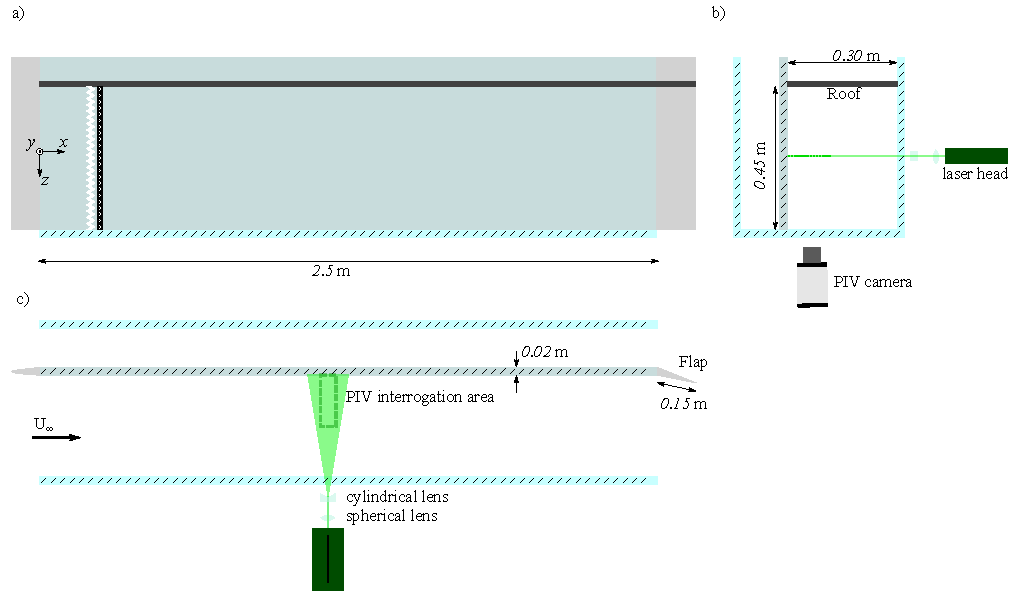
\includegraphics[width = 0.99\linewidth]{Figures/setup.pdf}
\caption{Sketch of the experimental setup. The flat plate is indicated in cyan, the walls of the water tunnel in light blue, and the 3D printed leading edge and flap in grey. a) Frontal view with reference system. The zig-zag tripping and dymo strips are included for reference. b) Lateral view, with illumination and imaging system. c) Top view, with optical arrangement and PIV measurement area.
}\label{fig:expsetup}
\end{figure}



An experimental campaign is held in the water tunnel at Universidad Carlos III de Madrid. The facility has a rectangular test section ($500 \times 550$~mm$^2$) with a length of $2.5$~m. A sketch of the experimental setup is reported in Figure~\ref{fig:expsetup}.  A flat plate is vertically mounted in the water tunnel, spanning the entire test section length. The flat plate is equipped with additively-manufactured leading edge of ratio 5:1 and trailing-edge flap of 150~mm chord to ensure the location of the stagnation point. The boundary layer is tripped 0.1~m downstream of the leading edge with a zig-zag turbulator of $1.5$~mm height, followed by a V-embossed tape which has a nominal height of 0.3 mm. The measurements are conducted at a single streamwise station located at approximately $x=1.1$~m from the leading edge. A characterisation of the turbulent-boundary-layer behaviour has been conducted to ensure that a nearly zero-pressure-gradient condition is achieved, and that the boundary layer is well-behaved in the location of the measurement \citep{Sanmiguel:2017JFM}. For such purpose, the working-fluid viscosity is characterised with an Ostwald viscosimeter calibrated with distilled water. Viscosity is measured several times in order to reduce as much as possible the random uncertainty, with a standard deviation below 0.5\%.

The setup for PIV measurements is sketched in Figure~\ref{fig:expsetup}b-c. The flow is seeded with neutrally-buoyant polyamide particles ($10$~$\mu m$ diameter). Illumination is provided by a dual cavity Nd:Yag Quantel Evergreen laser ($200$~mJ/pulse at $15$~Hz), shaped into a laser sheet with thickness of $1$~mm. A 5.5 MPixels Andor sCMOS camera is equipped with a $50$~mm and a $100$~mm lenses to capture two datasets with different resolution (respectively about 25~pix/mm and 65~pix/mm, corresponding to a magnification of 0.16 and 0.42 and an inner-scaled resolution of 0.52~pix/$\ell^*$ and  1.34~pix/$\ell^*$). The two datasets will be referred in the following as low-resolution (LR) and high-resolution (HR) dataset. In the LR dataset a region of $300 \times 1650$ pixels is imaged, corresponding to $ 12 \times 66$~mm$^2$. For the HR dataset the image format was $300 \times 2450$ pixels, corresponding to about $ 4.6 \times 38$~$mm^2$. For both datasets the streamwise extension of the imaged domain is sufficiently small (less than $\delta/2$) to ensure statistical homogeneity (thus allowing averaging in the streamwise direction), while the wall-normal size of the field of view is larger than $\delta$, thus ensuring a robust measurement of the freestream and a full-view of the velocity profile. 

In both cases 28.000 images are captured, with a particle image density of approximately $1.6\cdot10^{-3}$ and $0.5\cdot10^{-3}$ particles per pixel for the LR and HR dataset, respectively. The relatively low seeding density ensures that the probability of spurious particle pairing and the errors due to particles overlap are minimised. Nonetheless, the strong velocity gradients in the near-wall region combined with the limited image density reduce the robustness of the predictor in the near-wall region, thus reducing the number of paired particles.  

\begin{figure}
    \centering
    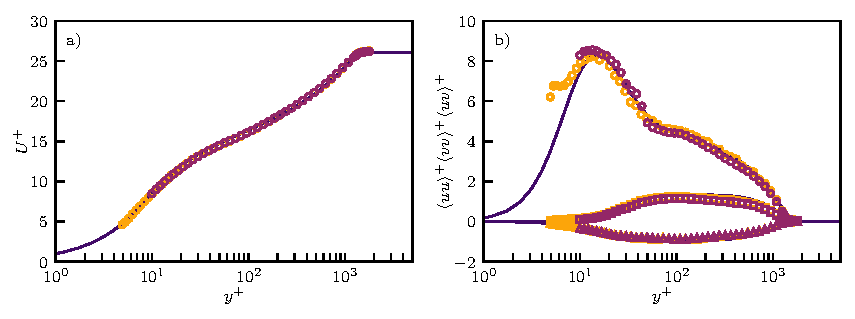
\includegraphics[width=\textwidth]{Figures/figure04.pdf}
    \caption{Profiles of the inner-scaled (a) mean velocity, and (b) Reynolds stresses of the velocity fluctuations. Colours refer to DNS \lcap{-}{dark}, EPTV - LR \lcap{-}{orange}, and EPTV - HR \lcap{-}{yellow}. In (b), symbols refer to streamwise \sy{black}{o}, wall-normal \sy{black}{s}, and shear \sy{black}{t} stresses.}
    \label{fig:F2_EPTVvsDNS}
\end{figure}


\subsection{Data processing}
A preprocessing is performed to remove the background and the laser reflection; the procedure is based on the eigenbackground subtraction described by \citet{Mendez2017181}. A super-resolution approach \citep{keane1995super} is followed to pair particle images in the captured dual-frames. The predictor velocity fields are obtained through image digital correlation \citep{willert1991digital}, based on a multi-pass \citep{soria1996investigation} image deformation algorithm \citep{scarano2001iterative} with a B-spline interpolation \citep{Astarita2005}. The final interrogation window is equal to 32 pixels with 75\% overlap region. Particle locations are identified with local maxima identification and Gaussian interpolation of the peak to achieve sub-pixel accuracy. The thresholding to identify whether a local maximum is a genuine peak is based on image statistics - only peaks above the local mean intensity plus one standard deviation are retained in the process. Particle images are then paired using a Kd-tree algorithm \citep{Tagliasacchi2021} for efficient pairing, with search biased by the PIV predictor. 

\subsection{EPTV and data post-processing} \label{ss:EPTV}
The ensemble averaging of the EPTV process is carried out on rectangular windows, with width of $200$ pixels and height variable between $3$ and $32$ pixels. A preliminary inspection of the wall reflection on the image allows to identify any misalignment between the camera reference system and the wall, and rotate the velocity vectors and averaging bins accordingly. Since the typical error in identifying manually the wall-position is of the order of the pixel size, the uncertainty of this procedure is below 0.5 degree.

On the streamwise direction an overlap of $80\%$ between the averaging windows is adopted. In the wall-normal direction initially a logarithmic grid has been adopted, with $50$ points from $1$ pixel above the wall up to $300$ pixels from the top of the image. In the last $300$ pixels a linear spacing has been adopted to obtain a robust estimate of the freestream. The profiles to be fitted with the composite profile are computed by averaging in the streamwise direction. A preliminary computation of the statistics has been carried out with the composite profile on the cases with window of $200\times3$ pixels (from now on named the reference cases for the LR and HR datasets using the full set of 28000 images). The results for the reference TBL are reported in Table~\ref{tab:1}. Additionally, the experimental reference cases are depicted in Figure~\ref{fig:fig01} against DNS data. 

The data are interpolated on a common grid based on the estimated $Re_\tau$ and wall position. The common grid is based on 70 logarithmically-spaced points from 0.1 wall units to {$0.9Re_\tau$},
and 20 linearly-spaced points from $0.93\delta$ to $1.3\delta$. This ensures that effects due to grid differences between the two datasets are removed.

The statistics computation is carried out by straightforward extraction of the statistical moments with equal weights on all vectors within the bin. While the polynomial approach by \citet{aguera2016ensemble} will improve the results close to the wall, it would not be comparable with the uncertainty estimation method presented in the previous section. Since the object of this work is to demonstrate the capability of our method to predict the uncertainty of the turbulent boundary layer parameters, we leave this aspect for future investigation.


\begin{figure}
    \centering
    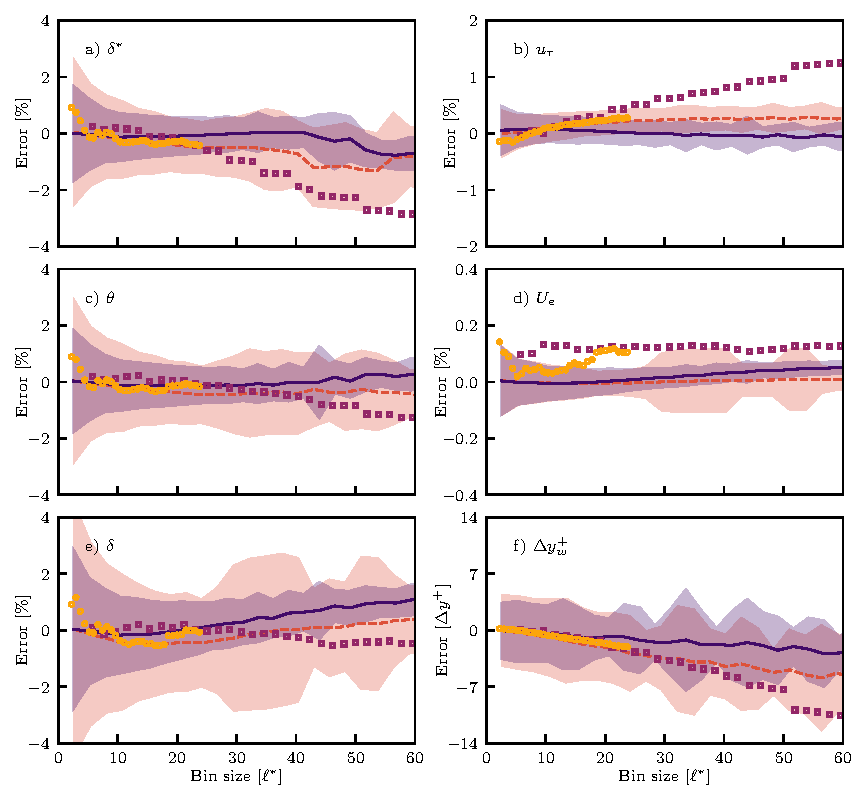
\includegraphics[width=\textwidth]{Figures/figure11.pdf}
    \caption{Comparison of error with respect to window size for a) displacement thickness, b) friction velocity, c) momentum thickness, d) freestream velocity, e) boundary layer thickness, and f) y origin. Symbols refer to DNS \lcap{-}{dark}, {Composite-profile} \lcap{--}{purple}, EPTV - LR \sy{orange}{s}, and EPTV - HR \sy{yellow}{o}. Error bars in DNS and {Composite-profile} refer to 3$\sigma$.}
    \label{fig:fig01}
\end{figure}


\subsection{Results}
\label{ss:expresults}

To compare the results among the experimental and the synthetic cases, the calculation of the profiles for the synthetic profiles has been carried out by setting the same resolution of the experiments. The averaged profiles are interpolated in the common grid described in \S\ref{ss:EPTV} to ensure the elimination of error sources due to grid differences between experimental and synthetic data.
Additionally, the estimation of TBL parameters is now performed by adding the random errors to the velocity profile and the {wall-normal} component. A total of 2000 runs are performed, and the standard deviation for each computed parameter is quantified to determine the corresponding uncertainty bars. 

The random error due to convergence is introduced as described in \S.\ref{ss:synthetic_method}, according to Eq.~\ref{ruido}. The TBL parameters are then computed using 2000 and 5000 images for the LR and HR dataset. The number of vectors $N_v$ is set equal to $350\cdot w$, with $w$ being the averaging bin size, to match the number of vectors observed in the dataset. The error of the experimental data is then estimated by using as a reference the velocity profile obtained using the full dataset of 28.000 images with window size of $200\times3$ pixels.

In Figure \ref{fig:F2_EPTVvsDNS} a comparison among the two experimental cases described in \S\ref{s:validation} and the DNS profile used as synthetic data is shown. Both experimental cases show an excellent agreement not only in the mean streamwise velocity profile (Figure \ref{fig:F2_EPTVvsDNS}a) but also in the different Reynolds stress components  (Figure \ref{fig:F2_EPTVvsDNS}b) up to the near-wall peak. For the high-resolution EPTV case, a deviation in the inner peak is appreciated which can be attributed to the residual reflections on the experimental images \citep{SanmiguelVila2017}. 

Figure \ref{fig:fig01} shows the relative error in the different boundary-layer parameters as a function of the bin size expressed in inner units. To normalise the error contribution, the resulting values of the {boundary-layer} quantities after fitting the original DNS profile, the Chauhan composite profile and the mean velocity profiles calculated using the full image data dataset (28.000 images) are employed. For the case of the quantities obtained by means of the composite profile proposed by \citet{Chauhan:2009p10824}, $u_\tau$ and $\Delta y^+$, it is observed for both quantities an error behaviour which, as expected, is equivalent to the error curves observed when analysing the effect of the first $y_0^+$ point available in hot-wire measurements \citep{Chauhan:2009p10824,Orlu:2010p36071,Rodriguez-Lopez2015}. For bin size values up to $\approx 12^+$, the error in both quantities is relatively small compared with the reference employed which is associated with profiles that have a $y_0^+<10$. When this bin size is exceeded, the error for both experimental cases shows much larger values. This effect is probably related to the higher levels of error in the logarithmic region for the experimental cases compared to the synthetic cases{, i.e. due to the strong local velocity profile curvature the PIV predictor for particles pairing is more prone to error}. For the quantities obtained by using the composite profile of \citet{Nickels:2004p15662} $\delta$, $U_e$, $\delta^*$ and $\theta$, the error curves are more robust and the agreement between the experimental data and the synthetic data is observed up to a bin size value of $\approx 25^+$. This corresponds to the location where there is no more inner points available and therefore all the estimation is performed based on the buffer and logarithmic region. It has to be noted that $U_e$ is slightly shifted in the error curves with respect to the reference. %As a consequence of the large number of images employed in the reference case (28.000), a more converged $U_e$ value is obtained compared to the error points which are calculated with only 2.000 images and therefore are more likely to be affected by the freestream disturbances.
This systematic error is quite small and might be to other minor issues, such as small drift of the flow conditions over the test time.

\section{Conclusions}

A method to estimate the uncertainty of {ZPG-}TBL parameters with the composite-profile based on data from full-field EPTV has been assessed. The proposed method is based on using data from simulations or composite profiles to reproduce the errors due to {wall-position} identification uncertainty, finite spatial resolution due to bin averaging and convergence due to finite number of samples. The synthetic and experimental validation demonstrate that the errors and uncertainty estimated using high-fidelity simulations and the composite-profile formulation are in good agreement, and predict accurately the range of error to be expected in the corresponding experiments. Simulation data can be more precise in determining the convergence limits since the streamwise velocity variance profile is well defined; on the other hand the approach based on the composite profile is more flexible, since it guarantees the possibility to closely match all the experimental conditions, including the Reynolds number.

The proposed approach can be used to:
\begin{enumerate}
    \item investigate systematic errors (as in \S\ref{s:SyntheticValidation}) by reproducing the same conditions to be expected in the experiments in terms of resolution and window size. It can be thus a useful tool to identify the requirements in terms of imaging before the experiments, and in principle it could also be used to reduce systematic errors.
    \item estimate the uncertainty range for the ZPG-TBL parameters. In this case, in addition to the spatial resolution and window size, the number of vectors per bin should also be included in the analysis to address errors due to convergence of the statistics. In this sense, this approach can be used also as an \textit{a priori} inference of the uncertainty, thus being useful to relate it quantitatively with the bin size and the number of vectors contained in it.
\end{enumerate}

\noindent{}It has to be remarked that this study is not including other sources of uncertainty which might be larger in an experiment than those quantified here, such as, for example, the uncertainty on the optical magnification. Furthermore, any departure from the condition of well-behaved ZPG TBL will determine additional uncertainty related to the suitability of the composite profile to fit the velocity profile. This is particularly delicate for quantities that are more sensitive to the quality of the near-wall region, such as $u_\tau$ or the wall position. 
Nonetheless, if any independent assessment of such additional uncertainty is available, the outcome of the uncertainty estimation approach proposed here can be used as input for the computation of combined uncertainties. \\

\section*{Code availability}
{The MATLAB\textregistered  codes for the calculation and plotting of the presented results are available from the repository \url{github.com/eaplab/EPTVuncertainty.git}. Camera-ready version of the figures have been generated with \url{github.com/guemesturb/TheArtist.git}.}

\section*{Acknowledgements}
RC, CSV and SD were partially supported by the Grant DPI2016-79401-R funded by the Spanish State Research Agency (SRA) and European Regional Development Fund (ERDF).